Para esta etapa del proyecto se detectarán los bad smells del código existente del pro proyecto y se aplicarán técnicas de refactoring e ingeniería para resolverlos.

\section{Revisión de los Shared Layout de las vistas}
\subsection{Librerías de terceros innecesarias}
\begin{itemize}
	\item \textbf{Síntoma:} Existen librerías de terceros procedentes de la plantilla que no se utilizan en ningún momento.
	\item \textbf{Solución:} Revisar que librerías se están usando dentro del proyecto. 
	\item \textbf{Procedimiento:} Se eliminó la carpeta que contenía los elementos de la plantilla, se migraron los paquetes a bower y se reciclo las hojas de estilos. Además, se escribió comentarios indicando la función que cumple cada uno.
\end{itemize}

\begin{lstlisting}[language=html]
@* CSS *@
<!-- Fuentes -->
<!-- Plugins -->
<!-- Bootstrap -->
<link href="~/lib/bootstrap/dist/css/bootstrap.css" rel="stylesheet" /> 
 <!-- Mensajes emergentes -->
<link href="~/lib/toastr/toastr.css" rel="stylesheet" />
<!-- Iconos -->
<!-- Iconos principales -->
<link href="~/lib/fontawesome/css/font-awesome.css" rel="stylesheet" /> 
<!-- Estilos de la aplicacion -->
<!-- Normalizacion de elementos -->
<link href="~/css/components.css" rel="stylesheet" /> 

@* JavaScript *@
<!-- jQuery -->
<script src="~/lib/jquery/dist/jquery.min.js"></script> 
<!-- Bootstrap -->
<script src="~/lib/bootstrap/dist/js/bootstrap.min.js"></script> 
<!-- Waypoints: Trigger para iniciar funcion -->
<script src="~/lib/waypoints/lib/jquery.waypoints.min.js"></script> 
\end{lstlisting}

\subsection{Error en la carga de las vistas}
\begin{itemize}
	\item \textbf{Síntoma:} Las vistas de la aplicación presentan un ligero retardo al cargar la data.
	\item \textbf{Solución:} Revisar las directivas de Angular. 
	\item \textbf{Procedimiento:} Se agregó la directiva ng-cloak
\end{itemize}

\begin{lstlisting}[language=html]
<div class="row" ng-app="app" ng-controller="alumnosController as vm">
	<wait-cursor display-when="vm.isBusy"></wait-cursor>
	<!-- Tabla de visualizacion -->
	<div ... ng-cloak>
		...
	</div>
</div>
\end{lstlisting}

\subsection{Error en la carga de las vistas}
\begin{itemize}
	\item \textbf{Síntoma:} Los archivos javascript de la aplicación están mezclados con los controladores angular.
	\item \textbf{Solución:} Colocar todos los controladores dentro de una carpeta.
	\item \textbf{Procedimiento:} Se creó la carpeta ``angular" para trasladar los controladores y se cambió la ruta de los paquetes en las vistas.
\end{itemize}

\begin{figure}[h]
	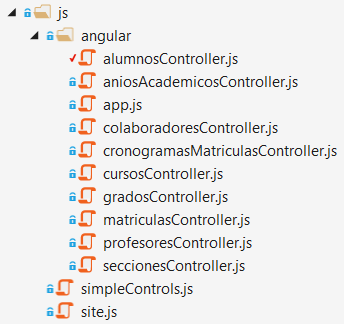
\includegraphics[width=0.5\textwidth]{1.png}
	\centering
\end{figure}

\begin{lstlisting}[language=html]
@section scripts {
	...
	<script src="~/js/angular/app.js"></script>
	<script src="~/js/angular/alumnosController.js"></script>
	...
}
\end{lstlisting}

\subsection{Validación de los nested objects}
\begin{itemize}
	\item \textbf{Síntoma:} El controlador no valida los nested objects.
	\item \textbf{Solución:} Crear una clase que realice este proceso iterativamente.
	\item \textbf{Procedimiento:} Se creó dos clases, una llamada ``CompositeValidationResult" y la otra ``ValidateObjectAttribute" que agregan un atributo a los decoradores de validación del modelo para que puedan usarse en todos los DTO.
\end{itemize}

\begin{figure}[h]
	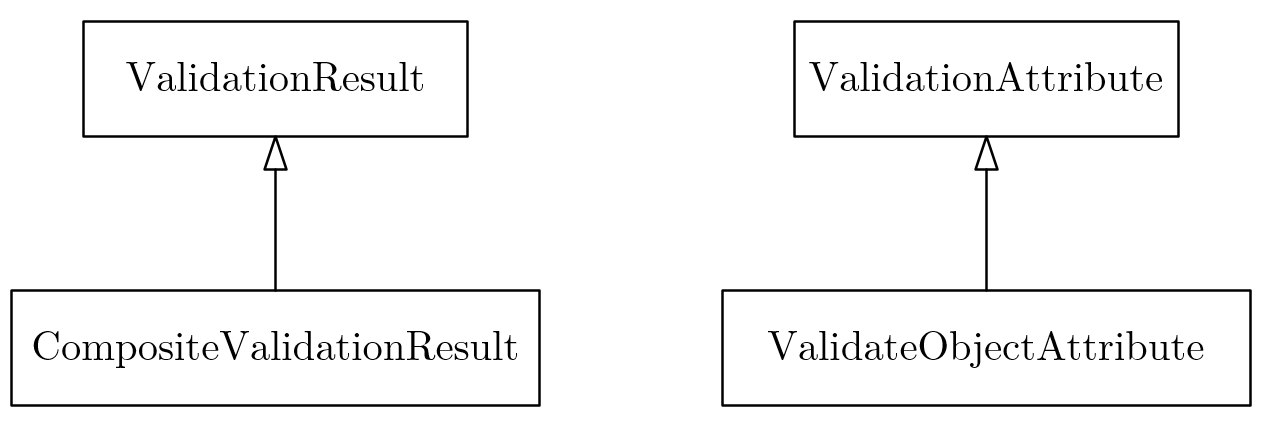
\includegraphics[width=0.7\textwidth]{2.png}
	\centering
\end{figure}

\begin{lstlisting}[language={[Sharp]C}]
public class AlumnoViewModel
{
	...
	[Required, ValidateObject]
	public virtual ApoderadoViewModel Apoderado { get; set; }
	...
}
\end{lstlisting}

